\documentclass[../main.tex]{subfile}
% \graphicspath{{\subfix{../images}}}
\begin{document}

\begin{figure}[bh]
    \centering
    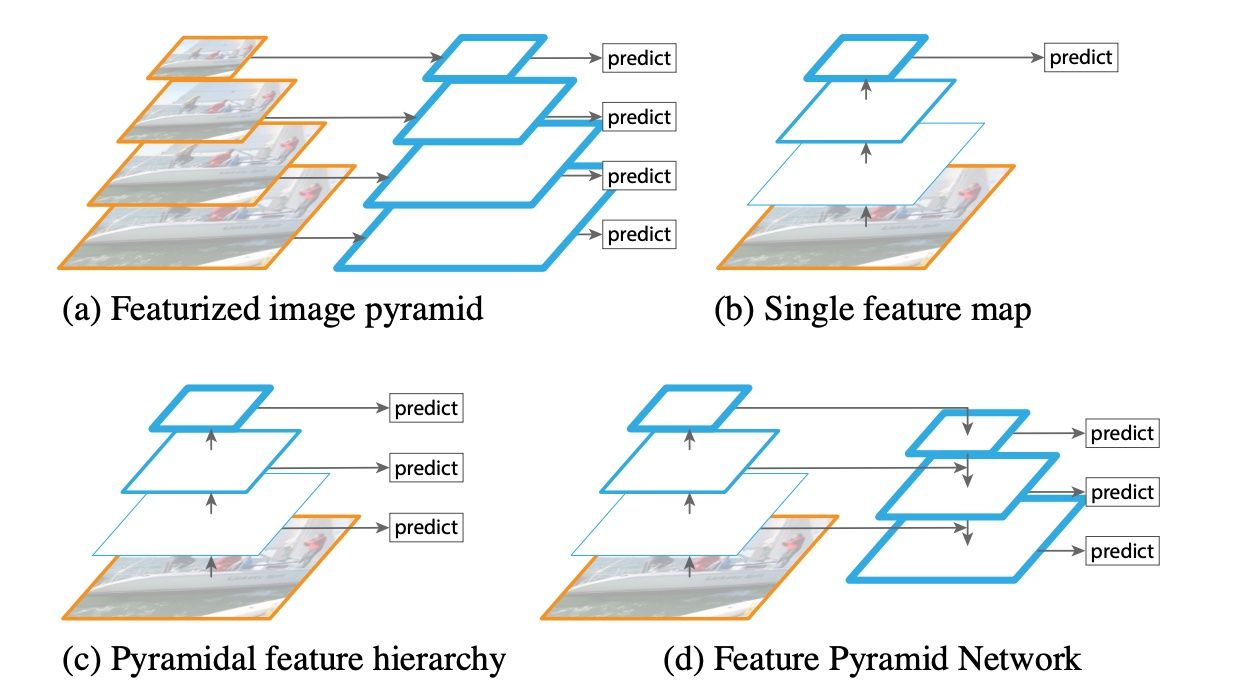
\includegraphics[width=.8\textwidth]{../images/img1.jpg}
    \caption{(a)使用图片金字塔来构建特征金字塔。特征在每个图片尺度上被独立计算,这是很慢的。(b)最近的检测系统选择使用单一尺度特征来进行更快的检测。(c)一个可选方案是复用卷积网络计算得到的金字塔特征层级并将之视作特征化图片金字塔。(d)我们提出的FPN和(b)(c)一样快,但是更加准确。在这张图中,特征图被标记为蓝色外边框,更粗的边框表示语义更强的特征。}
    \label{fig:img1}
\end{figure}


识别不同尺度的物体时计算机视觉中的一个基本挑战。构建在图片金字塔上的特征金字塔是标准解法的基础\cite{pyramid}(图\ref{fig:img1}(a))。在物体的尺度变化会通过移动它在金字塔中层级来补偿的角度来说,这些金字塔是具有尺度不变性的。直觉上来说,通过让模型扫描各个位置和各个尺度,模型可以在很大的尺度区间中检测物体。

在手工设计特征的时代,特征化的图片金字塔被重度使用。它们如此重要,以至于例如DPM的物体检测器要求密集尺度采样来达到好的结果(例如,在每个八度采样10个尺度)。对于识别任务,手工设计特征已经被深度卷积网络计算的特征大量替代。随着表示高层级语义的能力而来的,还有对于尺度变化的鲁棒性,因此似的根据在单一输入尺度计算的特征上识别更加简单(图\ref{fig:img1}(b))。然而即使有了如此的鲁棒性,为了得到最精准的结果我们仍需要金字塔。近期ImageNet和COCO检测挑战中的所有的顶部条目都在特征化的图片金字塔上进行多尺度测试(例如,\cite{16,35}。特征化图片金字塔中的每一个层级的主要优势在于它产生了一个包括高分辨率层级在内的所有层级语义都很强的多尺度特征表示。

然而,特征化图片金字塔中的每一个层级有着明显的局限。推理时间显著增加(例如在\cite{4}中增加4倍),这使得这个方法对于实时应用来说不切实际。不仅如此,就内存来说,在一个图片金字塔上端到端地训练一个深度网络是不切实际的,如果要使用的话,只能在测试阶段使用图片金字塔,而这制造了训练和测试时推理的不一致性。处于这些原因,Fast R-CNN和Faster R-CNN在默认设置下选择不适用特征化的图片金字塔。

然而,图片金字塔并不是计算多尺度特征表示的唯一方法。深度卷积网络会一层接着一层地计算一个\textit{特征层级},同时由于下采样层的存在,特征层级有一个固有的多尺度金字塔的形状。这个网络中特征层级产生了一系列有不同空间分辨率的特征图,然而也引入了由于不同深度产生的巨大语义缺口。高分辨率特征图有低层级特征,这损害了它们对于物体检测的表征能力。

Single Shot Detector(SSD)是最早进行将卷积网络的金字塔特征层级作为特征化图片金字塔尝试的检测器之一(图\ref{fig:img1}(c))。在理想情况下,SSD风格的金字塔可以复用在前向传播过程中各层计算的多尺度特征图,因此这是没有代价的。但是为了避免使用低层级特征,SSD放弃了复用已经计算好的各层,而是从网络的高层(例如VGG网络中的conv4\_3)开始并加入一些新层来构建金字塔。因此它错过了使用特征层级中的更高分辨率的特征图的机会。我们发现这对于检测小物体是十分重要的。

这篇文章的目标是自然地借助卷积网络的特征层级的金字塔形状同时构建一个在所有尺度都有强语义的特征金字塔。为了实现这一目标,我们借助通过自顶向下通路和旁路连接,将低分辨率强语义特征和高分辨率弱语义特征结合起来的结构(图\ref{fig:img1}(d))。结果是一个从单一输入图片尺度快速构建,然而在所有层级都有丰富语义的特征金字塔。换一种说法,我们展示了如何在不牺牲表征能力、速度和内存的情况下,构建一个可以替代特征化图片金字塔的网络内特征金字塔。

\begin{figure}[bh]
    \centering
    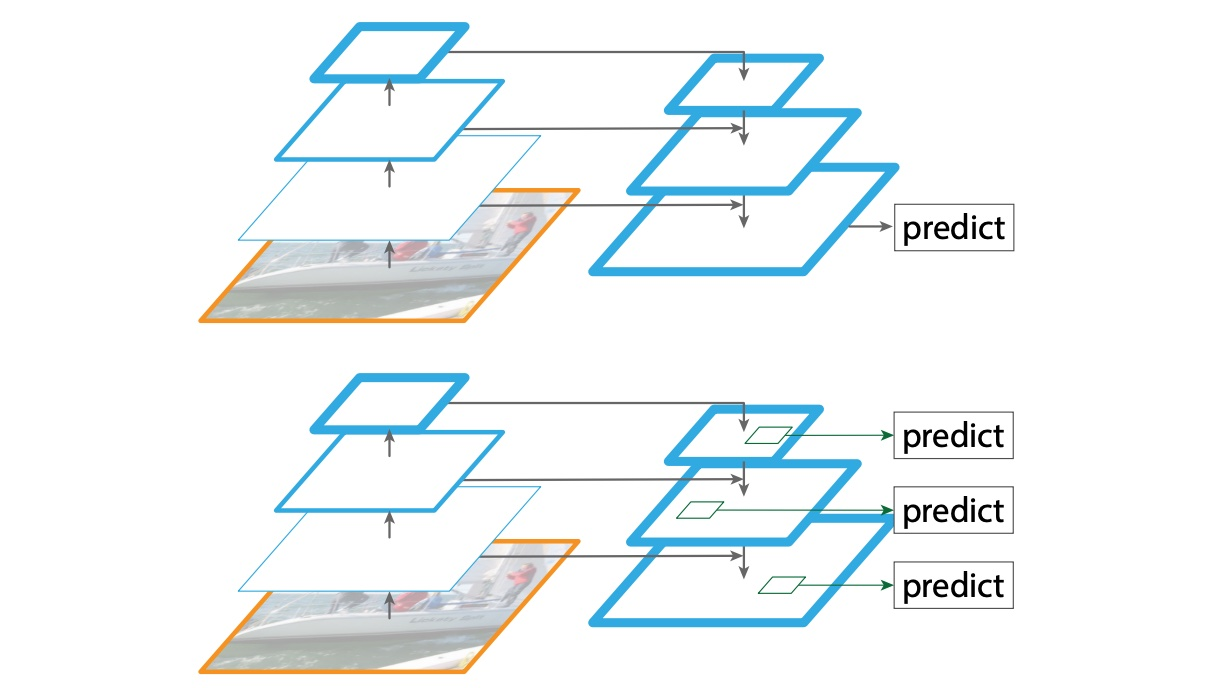
\includegraphics[width=.8\textwidth]{img2.jpg}
    \caption{顶部:有跳跃连接的自顶向下结构,仅在最好的层级预测(例如\cite{28})。底部:我们的模型与之有类似的结构但是借用它为\textit{特征金字塔},在所有层级独立做出预测。}
    \label{fig:img1}
\end{figure}

类似采用自顶向下以及跳跃连接的结构在最近的研究中十分普遍。它们的目标是产生分辨率良好的单一高层级特征图,并在其上进行预测(图\ref{fig:img2}顶部)。与之相反的是,我们的方法利用如特征金字塔的结构,并独立在各个层级进行预测(例如物体检测)(图\ref{fig:img2}底部)。我们的模型与特征化图片金字塔类似,这并没有在这些工作中被探索。

我们我们在多个检测和分割网络\cite{11,29,27}中评估了我们的方法,我们将之命名为Feature Pyramid Network (FPN)。在没有任何花里胡哨的情况下,我们简单地基于FPN和Faster R-CNN检测器,在COCO检测基准上达到了最好的单模型结果,超越了所有已有的重度手工设计的单模型条目。在消融实验中,我们发现在强大的单尺度ResNets Faster R-CNN基线上,FPN为候选边界框生成提高了8\%地平均召回率(Average Recall,AR);对于物体检测,它提高了2.3\%的COCO风格AP和3.8\%的PASCAL风格的AP。我们的方法也可以轻易地扩展到掩码候选,并提高了严重基于图片金字塔的最优方法地速度和实例分割AR。

额外地,我们的金字塔结构可以多尺度端到端训练,因此在训练和测试时是具有一致性的,若使用图片金子塔这将是不可能的。作为结果,FPN可以达到比已有最佳方法都更高的准确率。不仅如此,这种进步是在不增加单尺度基线的测试时间的条件下达到的。我们相信这些进步将会帮助未来的研究和应用。我们的代码将会开源。

\end{document}